\documentclass[12pt,a4paper]{paper}


\newcommand{\Title}{Analyse du cycle de vie du parc informatique de l’ENSEIRB-MATMECA} 
\newcommand{\Course}{Développement durable et responsabilité sociétale
\\ Département Informatique
\\ S6 - Année 2024/2025} 
\newcommand{\Author}{Mélissa Colin - Noé Offredo}
\newcommand{\Date}{\today}
\pagestyle{fancy}
\lhead{\textbf{\Author}} 
\rhead{1A - Informatique}
\cfoot{\thepage/\pageref{LastPage}}

% \fancypagestyle{plain}{ % Apply the fancy style to plain pages like the title page
%     \lhead{\textbf{\Author}} 
%     \rhead{1A - Informatique}
%     \cfoot{\thepage/\pageref{LastPage}}
% } POUR AVOIR COMME SYR LES LIVRES


\title{\textbf{\Title}}

% plusieurs auteurs 
\author{M. Colin\textsuperscript{1}, N. Offredo\textsuperscript{1}\\[6pt]
\textsuperscript{1} ENSEIRB-MATMECA\\
}

\begin{document}

% A VOIR SI ON GARDE
% \begin{titlepage}
%     \centering
%     \vspace*{3cm}
%     {\Huge \textbf{\Title}}\\[1.5cm]
%     {\Large \textit{\Course}}\\[2cm]
%     \textbf{\Author}\\[1cm]
%     \Date\\
%     \vfill
%     
\includegraphics[width=0.3\textwidth]{logo.png}
%     \vspace*{1cm}
% \end{titlepage}
% --------------------

\maketitle

% \begin{resume}
% C'est mon résumé. Il doit occuper AU MAXIMUM une dizaine de lignes.
% \end{resume}

% \begin{motscles}
% Exemple type, format, modèle.
% \end{motscles}

% \begin{abstract}
% It's the English version of the abstract. Exactly as in French it must be short. It must speak of the same topics...  
% \end{abstract}

% \begin{keywords}
% Example, model, template.
% \end{keywords}


\section{Introduction}
\subsection{Contexte et motivation}
Alors que la transition énergétique est au coeur des préoccupations de notre société, il est indispensable de se pencher sur l'impact environnemental des technologies numériques. En effet, la fabrication et l'utilisation des équipements informatiques génèrent une empreinte carbone significative. Dans ce contexte, l'ENSEIRB-MATMECA, école d'ingénieurs spécialisée dans le numérique, s'interroge sur la durabilité de son parc informatique. Ce rapport vise à évaluer l'impact environnemental de deux solutions numériques : 600 ordinateurs Dell de type tour T1700/3620 et 600 Raspberry Pi 4 Rev B connectés à 6 serveurs Dell Precision 7920T.

% \subsection{Plan}
% \noindent \lipsum[1-2]

\section{Méthodologie}
L’objectif de notre étude est de comparer empiriquement l'impact environnemental de deux solutions pour le parc informatique de l'ENSEIRB-MATMECA : 600 ordinateurs et 600 Raspberry Pi connectés à 6 serveurs. Nous avons nous concentrer sur la fabrication et l'utilisation de ces équipements, en négligeant les écrans et les périphériques d'entrée. La fin de vie des équipements ne sera pas prise en compte dans cette étude en raison de la complexité de sa modélisation. L'unité fonctionnelle retenue est l'utilisation de 600 ordinateurs pendant 5 ans à l'ENSEIRB-MATMECA.\\
Nous décrivons ci-dessous les outils de modélisation utilisés, ainsi que les processus de fabrication et d'utilisation des ordinateurs et des Raspberry Pi. 

\subsection{Outils de modélisation et base de données}
Nous avons utilisé le logiciel openLCA pour modélisé les processus de fabrication et d'utilisation des ordinateurs et des Raspberry Pi. Cet outil permet de réaliser des analyses de cycle de vie (ACV) en intégrant différentes bases de données, dont ecoinvent~\cite{ecoinvent2024}. Ecoinvent est une base de données de référence pour l'analyse du cycle de vie, fournissant des données sur les processus industriels, les flux de matières et d'énergie, ainsi que les impacts environnementaux associés. C'est pour sa richesse et sa précision que nous avons choisi cette base de données pour notre étude.

\subsection{Ordinateur Dell de type tour T1700/3620}
Dans une premiers temps, nous avons modélisé l'impacte environnemental des ordinateurs Dell de type tour T1700/3620 présent dans le parc informatique de l'ENSEIRB-MATMECA. Nous décrirons ci-dessous les différentes étapes de la modélisation, en commençant par la fabrication des ordinateurs, suivie de l'emballage et du transport. 
\subsubsection{Composants}
Ces modèles, relativement équivalents, contiennent plusieurs composants essentiels à leur fonctionnement. Pour cela nous avons réalisé un \textit{processus}\footnote{Un processus dans openLCA est un ensemble d'activités qui transforment des matières premières en produits finis.} modélisant un ordinateur et y avons intégré les éléments suivants en fonction des indictaions fournies dans le sujet~\cite{TP2_ACV_ENSEIRB-MATMECA} pour le choix des processus de la base ecoinvent~\cite{ecoinvent2024} :
\begin{itemize}
    \item Le processeur : integrated circuit, logic type
    \item Le disque dur : Hard disk drive, for desktop computer
    \item L'alimentation : Power supply unit, for desktop computer
    \item Le lecteur/graveur CD/DVD : Disk drive, CD/DVD, ROM, for desktop computer
\end{itemize}
A cela, nous avons ajouté le chassis de l'ordinateur, la carte mère, la RAM et la carte graphique. Ces composants ne sont pas encore modélisé dans la base de données ecoinvent. Pour se faire nous avons utilisé les providers créés lors d’un projet 2020/2021 par des étudiants de 2A de la filière Électronique.\\
Nous avons définis l'ensemble de ces composants avec une quantitée de une unitée hors mis pour la RAM, après observation visuelle du contenu de l'ordinateur, nous avons déterminé qu'un ordinateur contenait 2 barrettes de RAM. Nous l'avons donc défini avec une quantité de 2 unités.
% [Bonus 1]. Détailler la modélisation de la carte mère. La critiquer.

% [Bonus 2]. Décrire le processus du châssis en détails. Le critiquer.

\subsubsection{Fabrication}
Nous avons par la suite intégré le processus d'assemblage de l'ordinateur. Nous avons pour cela considéré l'électricité produite en Chine, l'eau potable et son traitement.
Le sujet~\cite{TP2_ACV_ENSEIRB-MATMECA} nous précise que l'éléctricité putilisé pour l'assemblage correspond au processus ecoinvent \textit{electricity,
medium voltage} avec une quantitée de 2,767 kWh. \textcolor{blue}{[Bonus 3]}~Pour vérifier cette infromation, nous avons consulté le rapport \textit{Electronic Devices - Part III}~\cite{Lehmann2007} qui indique que la consommation d'énergie pour découper les plaques d'acier est de 0,277 KWh, 0,222 KWh pour le fraisage, et que l'éléctricité pour l'assemblage est de 2,222 KWh. En additionnant ces valeurs, nous obtenons une consommation totale de 2,721 KWh. Le rapport mentionne néanmoins que ses valeurs sont des moyennes et que leurs écart-type géométrique est de 95\% ce qui signifie que la consommation d'énergie peut varier considérablement en fonction des conditions de fabrication. Par conséquent, nous avons décidé de conserver la valeur de 2,767 KWh fournie dans le sujet car elle est tout tout de même proche de la valeur que nous avons calculée.\\
Pour l'eau potable, le sujet~\cite{TP2_ACV_ENSEIRB-MATMECA} nous indique que la valeur est de 1600kg. Nous avons donc utilisé le processus ecoinvent \textit{tap water} avec cette quantitée carelle est confirmée par le rapport \textit{Electronic Devices - Part III}\cite{Lehmann2007} qui indique que la consommation d'eau pour l'assemblage est de 1620kg, ce qui est très proche de la valeur fournie dans le sujet.\\
Pour le traitement de l'eau, nous avons utilisé le processus ecoinvent \textit{wastewater, unpolluted} avec une quantitée de -1,62m³ trouvée dans le rapport \textit{Electronic Devices - Part III}\cite{Lehmann2007}. Cette valeur est négative car elle est considérée comme un déchet et la base de données ecoinvent qui utilise la méthode \textit{Opposite Direction Approach} qui consiste à modéliser les flux de déchets en tant que flux négatifs. Cette approche permet de représenter le traitement des déchets comme une consommation négative de ressources, inversant ainsi le sens conventionnel des flux de matériaux. En conséquence, le processus de traitement de l’eau est modélisé avec une valeur négative, indiquant qu’il s’agit d’un rejet nécessitant un traitement, et non d’une ressource consommée. Cette méthodologie garantit que les impacts environnementaux du traitement des déchets sont correctement pris en compte dans l’analyse du cycle de vie~\cite{openLCATutorial2020}.

\subsubsection{Emballage}
Pour être transporté, l'ordinateur doit être emballé. Nous avons donc modélisé l'emballage de l'ordinateur en prenant en compte les éléments suivants :
\begin{itemize}
    \item L'emballage cartonné
    \item Les granulés de plastique pour tous les films plastiques
    \item La transformation du plastique (polypropylène) en film
\end{itemize}
Nous avons utilisé le processus ecoinvent \textit{corrugated board box} pour l'emballage cartonné avec une quantitée de 2,19kg (toujours d'après le rapport \textit{Electronic Devices - Part III}\cite{Lehmann2007}). Pour les granulés de plastique, nous avons utilisé le processus ecoinvent \textit{polypropylene,
granulate} avec une quantitée de 0,16kg. Enfin, pour la transformation du plastique en film, nous avons utilisé le processus ecoinvent \textit{polymer foaming} avec une quantitée de 0,16kg. Ces deux dernières valeurs sont également fournies dans le sujet~\cite{TP2_ACV_ENSEIRB-MATMECA}.

\subsubsection{Transport}
Nous considérons que l'ordinateur est transporté du site de fabrication au site d'utilisation en bateau (15 000 km) et en camion (1000 km en Chine et 1000 km en France). Pour cela nous avons alors utiliser le processus \textit{transport, freight, sea, transoceanic ship} pour la partie maritime et les processus \textit{transport, freight, lorry 16-32 metric ton, EURO5} avec pour provider \textit{market for $\cdots$ RER} et \textit{market for $\cdots$ RoW} respectivement pour la partie terrestre en Chine et en France. Nous avons utilisé l'unité \textit{km × kg} pour le transport maritime et terrestre, en estimant le poids de notre colis avec la somme des poids de l'ordinateur et de son emballage, soit 10,75kg.


\subsubsection{Création du processus}
Nous avons alors pu créer le processus \textit{Computer DELL T1700/3620} visible en figure~\ref{fig:computer-process} en intégrant l'ensemble des processus que nous venons de décrire. Nous complétons ce processus pour prendre en compte à la fois les 600 ordinateurs mais aussi leur consommation électrique selon les données fournies dans le sujet~\cite{TP2_ACV_ENSEIRB-MATMECA}. \textcolor{red}{voir si on detail ici ou pas}. Ainsi nous pouvons créer le \textit{product system}\footnote{Un product system est un ensemble de processus interconnectés qui représentent un système de produits ou de services. Il permet d'analyser les flux de matières et d'énergie tout au long du cycle de vie d'un produit.} associé et réaliser le calcul d'impact.




\begin{figure}[h!]%[htbp]
    \centering
    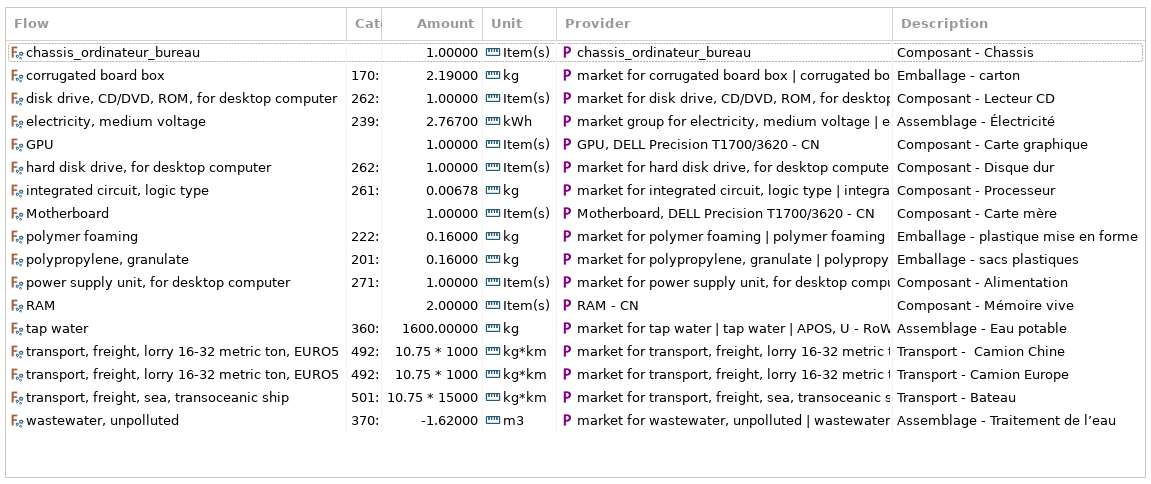
\includegraphics[width=\linewidth]{computer-process.png}
    \caption{Processus de fabrication de l'ordinateur}
    \label{fig:computer-process}
\end{figure}

\subsection{Six cent Raspberry Pi couplés à six serveurs}
Nous considérons dans notre étude que 600 Raspberry Pi 4 Rev B sont couplés à 6 serveurs Dell Precision 7920T. Nous allons modéliser l'impact environnemental de cette solution en utilisnat directement les processus qui nou sont été fournis. A partir de ces processus, nous avons pu créer le product system correspondant aux Raspberry Pi et aux serveurs. Nous avons ensuite modélisé la consommation électrique des Raspberry Pi et des serveurs en \textcolor{red}{COMPLETE STP}.

\section{Résulats}
\subsection{Ordinateur Dell de type tour T1700/3620}
\label{sec:computer}
\begin{figure}[h!]%[htbp]
    \centering
    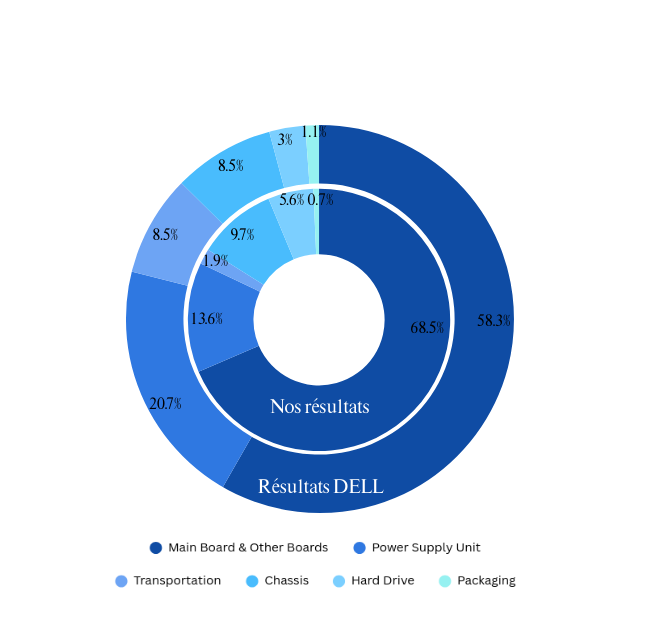
\includegraphics[width=\linewidth]{img/graph-dell-vs-our.png}
    \caption{Comparaison entre le bilan carbone de Dell et celui de notre modélisation}
    \label{fig:computer-impact}
\end{figure}
\textcolor{blue}{[Question 6-1]}~La figure~\ref{fig:computer-impact} présente la comparaison entre le bilan carbone de Dell et celui de notre modélisation. Nous pouvons observer que la carte représente près de 60\% du bilan carbone total d'après DELL, tandis que notre modélisation indique que la carte mère et les autres cartes représentent environ 70\% du bilan carbone total. Néanmoins ils sont équivalent en termes de CO\textsubscript{2}e émis comme présenté dans le tableau~\ref{tab:emissions}.\\
Nous avons également observé que le transport représente une part négligable d'après nos résultats, alors qu'il représente près de 10\% du bilan carbone d'après DELL. \\
Au total, nous avons obtenu un bilan carbone de 288,219 kg CO\textsubscript{2}e pour un ordinateur Dell de type tour T1700/3620, tandis que DELL annonce un bilan carbone de 341,544 kg CO\textsubscript{2}e.
\begin{table}[h!]
    \centering
    \begin{tabular}{|p{2.5cm}|p{2.4cm}|p{2.4cm}|}
    \hline
    \textbf{Composant} & \textbf{Émission d'après DELL} & \textbf{Émission d'après nos résultats } \\
    \hline
    Transportation & 28{,}89 & 5{,}421 \\ \hline
    Chassis & 28{,}89 & 28{,}075 \\ \hline
    Power Supply Unit & 70{,}62 & 39{,}076 \\ \hline
    Packaging & 3{,}852 & 1{,}997 \\ \hline
    Hard Drive & 10{,}272 & 16{,}149 \\ \hline
    Main Board \& Other Boards & 199{,}02 & 197{,}501 \\
    \hline
    \textbf{Total} & \textbf{341{,}544} & \textbf{288{,}219} \\
    \hline
    \end{tabular}
    \caption{Émissions de CO\textsubscript{2}e pour chaque composant de l'ordinateur Dell T1700/3620 selon DELL et selon nos résultats}
    \label{tab:emissions}
\end{table}
    
\subsection{Six cent Raspberry Pi couplés à six serveurs}
\textcolor{gray}{\lipsum[1-2] }

\subsection{Comparaison entre les 2 stratégies}

\textcolor{gray}{10. Vous pouvez maintenant effectuer une comparaison entre les 2 stratégies. Quelle est votre}
\textcolor{gray}{conclusion ? Quelles sont les limitations de l’étude ? Quels sont les avantages et les inconvénients}
\textcolor{gray}{de chacune des stratégies ?}
\textcolor{gray}{Point d’étape : appelez votre chargé·e de TP}
\textcolor{gray}{11. Six serveurs sont suffisants mais en cas de panne, cela peut poser problème. Que se passe-t-il}
\textcolor{gray}{si l’on en considère 8 ? Votre conclusion change-t-elle ?}
\textcolor{gray}{[Bonus 5]. Que se passe-t-il si l’on fait à présent notre étude avec le mix électrique polonais ?}
\textcolor{gray}{[Bonus 6]. Les écrans n’ont pas été modélisés. Quels sont les choix que nous aurions pu faire ?}
\textcolor{gray}{(Rechercher par exemple des bilans carbone d’écrans).}

\section{Discussion}
\subsection{Ordinateur Dell de type tour T1700/3620}
\textcolor{blue}{[Question 6-2]}~Dans la section~\ref{sec:computer}, nous avons pu constater que les empreintes carbones que nous avons calculées et celle fournie par DELL sont du même ordre de grandeur, bien que celle de DELL soit légèrement supérieure. Cette différence, principalement visible dans le transport, pourrait provenir d'une différence dans la façon de modéliser l'acheminement des ordinateurs. En effet, DELL indique que les ordinateurs sont assemblés en Europe, tandis que nous avons considéré celui-ci en Chine. Ce qui pourrait présenter des différences d'acheminement des composants par rapport à notre modélisation.
\textcolor{blue}{[Question 7]}~\textcolor{gray}{a. Bilan carbone : Comment se sépare la phase de fabrication de la phase d’usage ? Et par rap-}
\textcolor{gray}{port à l’étude de Dell ?}
\textcolor{gray}{b. Bilan carbone : Qu’est-ce qui est le plus impactant dans l’ordinateur ?}
\textcolor{gray}{c. Étudier d’autres facteurs d’impact comme par exemple : ionizing radiation, water consumption}
\textcolor{gray}{et mineral ressources scarcity.}


\subsection{Six cent Raspberry Pi couplés à six serveurs}

\textcolor{gray}{
On considère que 6 serveurs sont suffisants pour piloter 600 clients légers constitués de Raspberry
Pi.\\ 8. Regarder et commenter le processus Raspberry Pi 4 Rev B. Faire de même avec le processus
Serveur 48 cœurs. Remarque : Le processus mounting correspondant ici à l’assemblage des composants sur le circuit imprimé (placement des composants, brasure, nettoyage des cartes
assemblées à l’issue du processus, etc.). Pour l’ordinateur et le serveur, il est déjà directement intégré au niveau des composants.\\ 9. Créer le product system Use of Raspberry + Server at ENSEIRB-MATMECA. Ne pas oublier de prendre en compte la consommation électrique des Raspberry Pi mais aussi des serveurs. Répondre aux questions qui vous semblent pertinentes de la question 7 :}
\textcolor{gray}{a. Bilan carbone : Comment se sépare la phase de fabrication de la phase d’usage ? Et par rap-}
\textcolor{gray}{port à l’étude de Dell ?}
\textcolor{gray}{b. Bilan carbone : Qu’est-ce qui est le plus impactant dans l’ordinateur ?}
\textcolor{gray}{c. Étudier d’autres facteurs d’impact comme par exemple : ionizing radiation, water consumption}
\textcolor{gray}{et mineral ressources scarcity.}
\subsection{Comparaison entre les 2 stratégies}
\textcolor{blue}{[Bonus 4]}~\textcolor{gray}{[Bonus 4]. Bilan carbone : Quel est le bilan carbone d’un étudiant ou d’une étudiante de}
\textcolor{gray}{l’ENSEIRB-MATMECA pour la partie informatique durant ses 3 années d’études ?}
\textcolor{gray}{\lipsum[1-2] }
\subsection{Limites de l'étude}
\textcolor{blue}{[Question 10-1]}~L'ensemble des processus utilisé pour modélisé les ordinateur sont déjà intégrés dans la base de données ecoinvent. Cependant, il est important de noter que ces processus peuvent ne pas être entièrement représentatifs des modèles spécifiques de l'ordinateur Dell T1700/3620. Par conséquent, il est possible que les résultats de l'analyse de cycle de vie ne reflètent pas fidèlement l'impact environnemental réel de ces ordinateurs. De plus, la modélisation des Raspberry Pi et des serveurs a été réalisée en utilisant des processus génériques, ce qui peut également introduire des incertitudes dans les résultats. Il est donc essentiel d'interpréter les résultats avec prudence et de considérer ces limitations lors de l'évaluation de l'impact environnemental du parc informatique de l'ENSEIRB-MATMECA.
\textcolor{blue}{[Bonus 6]}~\textcolor{gray}{es écrans n’ont pas été modélisés. Quels sont les choix que nous aurions pu faire ?
(Rechercher par exemple des bilans carbone d’écrans).}
\subsection{Perspectives}
\textcolor{blue}{[Question 11]}~\textcolor{gray}{Six serveurs sont suffisants mais en cas de panne, cela peut poser problème. Que se passe-t-il si l’on en considère 8 ? Votre conclusion change-t-elle ?}
\textcolor{blue}{[Question 10-2]}~\textcolor{gray}{Quels sont les avantages et les inconvénients de chacune des stratégies ? \\ Six serveurs sont suffisants mais en cas de panne, cela peut poser problème. Que se passe-t-il si l’on en considère 8 ? Votre conclusion change-t-elle ?}

% Conclusion
\section{Conclusion et ouvertures}
\textcolor{gray}{\lipsum[1-2] }
% \include{glossaire}

% % Références
\printbibliography
\addcontentsline{toc}{section}{Références}
% \bibliography{bibliography}

\appendix

\end{document}
